\section{The performance-complexity trade-off problem}\label{sec:performance-complexity}

The main aim of this work is to explore the performance-complexity characteristics in the context of graph learning, as described for example by \cite{prochazka_downstream_2022}. Consider an undirected graph \( G \) with nodes \( V \left( G \right) \) and edges \( E \left( G \right) \). The result of the graph coarsening part of the algorithm is a sequence of graphs \( G_0, G_1, G_2, \dots, G_L \) where \( G_0 = G \) and \( L \in \mathfield{N} \) is a hyper-parameter of the method.
Given a model \( M \) that operates on graphs, a performance metric \( P \left( G, M \right) \) and a complexity metric \( C \left( G, M \right) \), the sequence \( G_0, G_1, \dots, G_L \) can be plotted in the performance-complexity space, where the original graph \( G_0 \) usually provides the best performance and incurs the most complexity and subsequent coarsened graphs improve complexity and hurt performance. -- see Figure \ref{fig:performance-complexity} for an illustration.

\begin{figure}
  \centering
  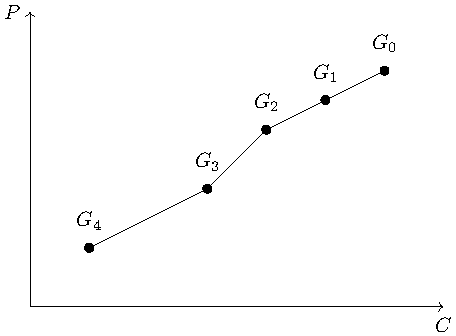
\includegraphics[width=0.45\textwidth]{images/performance-complexity/performance-complexity.pdf}
  \caption{An example of a performance-complexity curve for a sequence of graphs.}
  \label{fig:performance-complexity}
\end{figure}

This performance-complexity characteristics allows for a choice of an optimal \textbf{working point} for the model M - i.e., the choice of the optimal coarsening level \( G_i \), which directly influences both the performance and the complexity of the model. The choice of the working point is subjective and dependent on the particular use-case, downstream task and the environment in which the model is to be deployed. In general, however, two distinct uses of the characteristics emerge:
\begin{itemize}
  \item Finding the most performant model for a given complexity budget. That is, for a given maximum allowable complexity \( C_\mathrm{max} \), a graph \( G_i \) is to be found that maximizes \( P \left( G_i, M \right) \) while maintaining \( C \left( G_i, M \right) \leq C_\mathrm{max} \).
  \item Finding the least complex model satisfying a performance target. That is, for a given minimum acceptable performance \( P_\mathrm{min} \), a graph \( G_i \) is to be found that minimizes \( C \left( G_i, M \right) \) while maintaining \( P \left( G_i, M \right) \geq P_\mathrm{min} \).
\end{itemize}

\subsection{Choice of the performance and complexity metrics}

The choice of a suitable performace metric \( P \left( G, M \right) \) is dependent on the downstream task in question -- usually, the same metric used to evaluate the downstream model is utilized as the performance metric. In this work, the accuracy of the transductive classification is used as the chosen performance metric.

In practice, two of the most important complexity metrics are computational complexity and memory complexity. These may not only affect the monetary cost and time needed to train a model, but may prevent the application of a considered model or architecture outright due to the infeasibility of the given configuration. As shown in \cite{chiang_cluster-gcn_2019}, in the context of graph algorithms, a good proxy for the real-world complexity metrics may be the number of edges in a graph, or the number of nodes in the graph, which is the metric used in the rest of this work.

\subsection{Computational complexity of finding the optimal working point}

While the proposed methods may yield models and graphs with lower computational demands than models using the original graph, the algorithm for finding the optimal working point itself entails running the same complex models on multiple graphs, therefore potentially offsetting any gains from the lower complexity of the model itself. To overcome these potential shortcomings, the following options are considered:
\begin{itemize}
  \item The optimal working point may generalize to datasets other than the one used for the performance-complexity analysis. While this may not in general be said for any two datasets, similar datasets may arise in the practical setting, such as in the domain of computer network security, where a new graph is produced each time the network is scanned and it is reasonable to assume that the working point would be the same for graphs generated in this manner. Generally, this applies especially well in the case of transductive classification where the model needs to be re-trained when the underlying graph changes.
  \item The whole performance-complexity curve is not needed to choose the optimal working point. In the context of this work, the graphs are evaluated in reverse order, i.e. starting with \( G_L \). For both the case of a complexity budget and the performance target, the evaluation can be stopped when the bounding condition is fulfilled, therefore removing the need to evaluate the model on the graphs with the greatest complexity demands.
\end{itemize}
